\documentclass[11pt,a4paper]{article}
\usepackage[margin=2.5cm]{geometry}
\usepackage{amsmath,amssymb,array,graphicx,booktabs,siunitx,flafter,placeins,xcolor}
\usepackage[tableposition=top]{caption}
\usepackage[hidelinks]{hyperref}
\sisetup{detect-all,group-separator={\,},group-minimum-digits=4}
\setcounter{topnumber}{3}
\renewcommand{\topfraction}{0.85}
\renewcommand{\textfraction}{0.1}
\newcommand{\E}{\mathbb{E}}
\title{Demand Forecasting for a Giftware Wholesaler:\\From Transactions to Order
  Quantities}
\author{Immanuel Albrecht \and Claude Opus 5.5 (Anthropic)}
\date{November 2026}
\pdfinfoomitdate=1  % no creation/modification date in the PDF
\pdftrailerid{}
\begin{document}
\maketitle

% Structure: main text at most 10 pages, details in the appendix.
% Sections 8 and 9 written by Claude, reviewed by Immanuel Albrecht.

\section{Overview}
\label{sec:overview}

Abbreviations are listed in Appendix~\ref{app:glossary}.

A small online shop or wholesaler has to decide every week how much of each product to
reorder. This report documents a complete answer on real data: two years of
transactions of a UK giftware wholesaler are cleaned into a weekly demand panel, products are
segmented by value and demand pattern, and 25 forecasting methods, from moving averages to a
global LightGBM model with one model per quantile level, are compared on a rolling-origin
backtest with paired bootstrap confidence intervals. The forecast that the order decision
needs is not a single number but a set of quantiles, and for the order-up-to level the
quantiles of demand \emph{summed} over lead time and review period; Section~\ref{sec:paths}
builds these from sample paths. Section~\ref{sec:newsvendor} turns quantiles into order
quantities, and Section~\ref{sec:simulation} simulates a quantile-based order policy against
the rules a small shop would use, week by week over the test period, in pounds.

Every number comes from a run folder with its configuration, git commit and data version (a
hash of the cleaning configuration), the per-origin metrics and every evaluated forecast, so
each table can be reproduced from the repository. Model choices were made on 22 tuning origins
(January--May 2011); the 26 test origins (June--November 2011) were used once, at the end.

\begin{table}[ht]
  \centering
  \small
  \caption{Main results on the 26 test origins (June--November 2011), focus set of 748
    products, horizons 1--8 weeks. MASE and CRPS are scaled by each series' in-sample naive
    error; rcov = coverage of the central intervals under the randomised PIT
    (Section~\ref{sec:metrics}). The selected model per segment is the LightGBM quantile model
    in every focus segment, so ``best'' equals it on this set.}
  \label{tab:summary}
  \begin{tabular}{lrrrr}
    \toprule
    Model & MASE & CRPS & rcov 80\,\% & rcov 95\,\% \\
    \midrule
    Seasonal naive (lag 52) & 1.273 & 0.611 & 75.0 & 92.4 \\
    Naive (last week) & 0.822 & 0.448 & 80.5 & 94.6 \\
    Moving average, 4 weeks & 0.715 & 0.385 & 81.4 & 95.2 \\
    ETS (item) + MA(52) bulk & 0.715 & 0.355 & 82.5 & 94.9 \\
    LightGBM quantile models (selected) & \textbf{0.711} & \textbf{0.336} & 81.4 & 94.5 \\
    \bottomrule
  \end{tabular}
\end{table}

Against the two forecasting criteria set at the start: the selected model beats seasonal naive by
44\,\% in MASE on the focus set (paired bootstrap difference $-0.562$, 95\,\% CI
$[-0.611, -0.512]$), and its 80\,\% and 95\,\% intervals cover 81.4\,\% and 94.5\,\% of the
test outcomes, within $\pm 3$ percentage points of nominal under the randomised PIT. The
honest qualification: against a 4-week moving average the MASE gain is not significant
($-0.004$, CI $[-0.016, 0.008]$); the clear gain is in the quantiles (CRPS $-0.049$,
$[-0.059, -0.041]$), which is what the order decision uses.

That gain carries over to the decision. In a weekly simulation of the 748 products over the 26
test weeks, ordering up to a quantile of the sample-path sums needs 15--33\,\% less average
stock than the spreadsheet rule ``four-week mean times a buffer'' at the same fill rate, and at
the operating points fixed on the tuning weeks it serves more demand at a total cost 16--22\,\%
lower than the rule with a 100\,\% buffer (base costs), and at a lower cost under every lead time and cost assumption tried (Section~\ref{sec:simulation}).

\section{Data and cleaning}
\label{sec:data}

The data are the \emph{Online Retail II} transactions from the UCI Machine Learning Repository\footnote{Chen, D.\ (2012). \emph{Online Retail II} [Dataset]. UCI Machine Learning Repository. \url{https://doi.org/10.24432/C5CG6D}. Licensed under CC\,BY\,4.0, \url{https://creativecommons.org/licenses/by/4.0/}. Changes: cleaned and aggregated to weekly demand per product as described in this section; the raw files are not modified or redistributed.}: all
1\,067\,371 invoice lines of a UK online retailer of giftware from 1 December 2009 to
9 December 2011; many customers are wholesalers. Each line has invoice, stock code,
description, quantity, timestamp, unit price, customer id and country.

Cleaning is a sequence of rules, each a pure function with its own tests, and every rule books
the lines, units and revenue it removes. Raw totals reconcile exactly with the panel plus the
removals (Table~\ref{tab:cleaning}).

\begin{table}[ht]
  \centering
  \small
  \caption{Cleaning reconciliation (data version \texttt{ae898752}). Units removed by R5 are
    negative because stock adjustments carry negative quantities.}
  \label{tab:cleaning}
  \begin{tabular}{lrrr}
    \toprule
    Step & Lines & Units & Revenue (£) \\
    \midrule
    Raw (both sheets) & \num{1067371} & \num{10608492} & \num{19287251} \\
    R1 overlap of the two sheets & \num{22523} & \num{166648} & \num{377488} \\
    R4 non-product codes (postage, fees, \dots) & \num{5832} & \num{10438} &
      \num{-71536} \\
    R5 stock adjustments (price $\le 0$ etc.) & \num{5972} &
      \num{-320653} & 0 \\
    R6 order corrections & \num{5130} & 0 & \num{38350} \\
    R8 incomplete last week & \num{17585} & \num{162288} & \num{311735} \\
    R9 returns outside the active window & 293 & \num{-2450} & \num{-8727} \\
    \midrule
    Demand (panel) & \num{995125} & \num{10805429} & \num{18932649} \\
    Returns (separate panel column) & \num{14911} & \num{-213208} & \num{-292709} \\
    \bottomrule
  \end{tabular}
\end{table}

The decisions behind the rules: demand is \emph{gross orders}. A cancellation that exactly
undoes a sale of the same customer, product and quantity within seven days is an order
correction and removes both lines (R6); every other cancellation is a return, kept in its own
column and not subtracted from demand (1.5\,\% of revenue). Exact duplicate lines (11\,812
extra copies) were kept after both variants were built and compared: weekly totals move by
less than 1.5\,\%. Stock codes are upper-cased (R3); letter suffixes stay separate products.
Unusually large lines (quantity above median $+\,10$ MAD on the log scale) were reviewed by
hand in a small browser tool; none was removed (R7), because large wholesale orders are real
demand, but they shape the models (Section~\ref{sec:models}).

The panel has one row per product and ISO week: units, revenue, invoices, customers, median
price, the largest customer's share, returns and the number of trading days. Weeks between a
product's first and last sale are zero-filled; the two Christmas closures (weeks of
28 December 2009 and 27 December 2010) are \emph{missing}, not zero. The result is
\num{4718} products over 105 weeks (30 November 2009 to 28 November 2011).

\emph{Sales are not demand.} When the shop was out of stock, the data show only what it
could sell. Stock levels are not in the data, so sales are treated as demand throughout;
Section~\ref{sec:limitations} returns to this.

\section{Exploration and segmentation}
\label{sec:segments}

\begin{figure}[t]
  \centering
  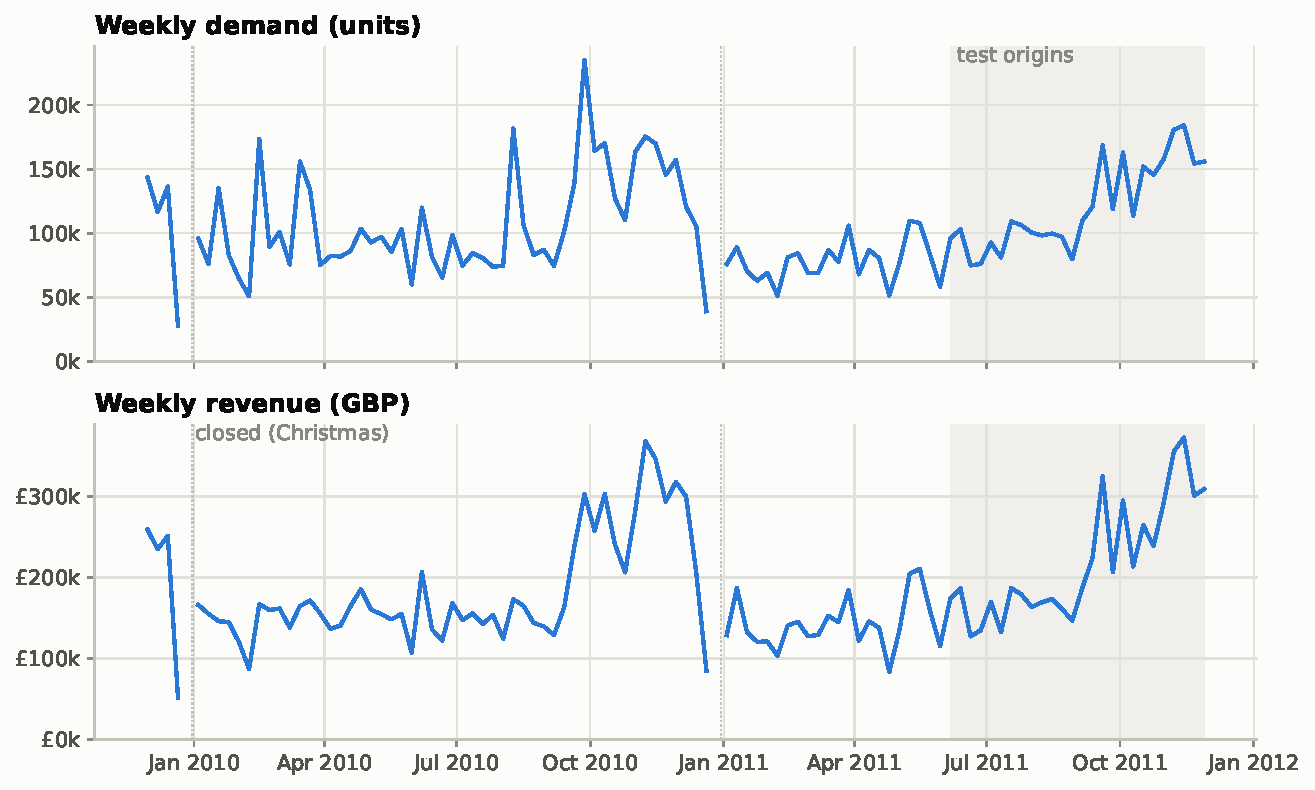
\includegraphics[width=0.85\textwidth]{figures/weekly_totals.pdf}
  \caption{Weekly demand and revenue; test origins shaded, Christmas closures dotted.}
  \label{fig:weekly}
\end{figure}

Demand is strongly seasonal (Figure~\ref{fig:weekly}): September to December bring 43\,\% of
the 2010 revenue, with the peak in November. The product range turns over quickly: products
first sold after the first quarter bring 33\,\% of all revenue, and 1\,567 products have not
sold in the last twelve weeks. All segments are computed on the weeks before the first test
origin (6 June 2011), so the test period never influences which products are studied.

\paragraph{ABC by revenue.} A = top 80\,\% of revenue (952 products), B = next 15\,\%
(1\,145), C = the rest (2\,047). Products with demand in a single week (162, 0.08\,\% of
revenue) get no segment.

\paragraph{Syntetos--Boylan classes.} The average inter-demand interval (ADI) and the squared
coefficient of variation of the non-zero weekly demand (CV$^2$), with the usual cut-offs 1.32
and 0.49, split products into smooth, erratic, intermittent and lumpy. A few wholesale customers
dominate many products (one customer buys more than half the units of 463 products); a single
pallet order turns a smooth series into an erratic one. The classes are therefore computed
without lines above ten times the product's median line quantity, which moves 336 products from
erratic to smooth (Figure~\ref{fig:sb} in the appendix).

\paragraph{Evaluation sets.} The \emph{focus set} is the 748 A products with at least 52
active weeks before the first test origin: 68.8\,\% of the revenue, mostly smooth (293) and
erratic (373), with 16 intermittent and 66 lumpy products. The \emph{full set} contains every
product with a sale before the forecast origin, about 4\,300 per origin, including products
without a segment (new, or with a single week of demand), labelled \emph{unclassified}. The original
design had A and B products in the focus set; with B included it would have had 1\,530 products,
mostly short or sparse series, and the A-only set was chosen instead.

\section{Backtest design and metrics}
\label{sec:metrics}

\paragraph{Origins and horizons.} Forecasts are made at weekly origins $t$ for the weeks
$t, t+1, \dots, t+7$ ($h = 1, \dots, 8$) from the data of the weeks before $t$ only; the
backtester hands models a history object that raises an error when a later week is read, and
a test with a ``cheating'' model checks this. Tuning origins: the 22 Mondays from
3 January to 30 May 2011; test origins: the 26 Mondays from 6 June to 28 November 2011,
including the Christmas build-up. Target weeks after the end of the data are not scored.
Each forecast has a mean and ten quantiles $\tau \in \{0.025, 0.05, 0.1, 0.2, 0.5, 0.8, 0.9,
0.95, 0.975, 0.99\}$; the 80\,\% interval is $[q_{0.1}, q_{0.9}]$, the 95\,\% interval
$[q_{0.025}, q_{0.975}]$.

\paragraph{Point and probabilistic metrics.} For a series with in-sample naive error
$s = \operatorname{mean}_{u<t} |y_u - y_{u-1}|$, MASE is the mean of $|y - \hat y|/s$ and the
scaled pinball loss at level $\tau$ is
\begin{equation}
  \rho_\tau(y, q) = \frac{1}{s}\bigl(\tau\,(y - q)^+ + (1 - \tau)\,(q - y)^+\bigr).
\end{equation}
with $(x)^+ = \max(x, 0)$. Twice the mean over the ten levels approximates the CRPS (scaled); lower is better, and a
point forecast scores on CRPS through its quantiles only. Bias is $\sum (y - \hat y) /
\sum y$ (positive = under-forecast). Every metric is reported unweighted and weighted by each
product's revenue in the 52 weeks before the origin.

\paragraph{Coverage of discrete demand.} With many zero weeks the lower quantiles are often
exactly 0, and then $y = q = 0$ counts as $y \le q$: the share of outcomes below $q_{0.025}$
is 19\,\% on the focus set even for a well calibrated forecast, and 56\,\% on the full set.
Coverage is therefore also reported under the \emph{randomised PIT}: where the outcome ties
with one or more quantiles, it is spread uniformly over the tied levels instead of counting as a
full hit (``rcov''). Both numbers are in the tables; the criterion uses rcov.

\paragraph{Comparisons.} Two runs are compared by a paired bootstrap over series (2\,000
resamples) of the per-series mean difference; differences whose 95\,\% interval contains 0 are
reported as not significant.

\section{Models}
\label{sec:models}

All models were developed on the tuning origins in experiments E1--E7; Table~\ref{tab:tuning}
in the appendix lists the tuning numbers. The main steps:

\paragraph{Baselines (E1, E2).} Naive, seasonal naive (lag 52), moving averages over 4, 8 and
13 weeks, and for intermittent demand Croston, SBA and TSB with $\alpha \in \{0.1, 0.2\}$.
Their quantiles come from empirical residual quantiles: the method's $h$-step errors on the last
52 weeks, divided by the series scale and pooled per segment and horizon. MA(4) was the best
baseline. The specialised intermittent methods did not beat it on the intermittent and lumpy
series; Croston and SBA keep forecasting a positive rate after a product's last sale, which is
why they fail badly on the full set.

\paragraph{Item and bulk demand (E2b).} Wholesale orders above ten times the product's median
line quantity carry 37\,\% of the units. Forecasting ordinary (``item'') demand and the bulk
rate separately, then adding them, improved the CRPS of every method (MA(4) item + MA(52) bulk:
focus CRPS 0.364 vs.\ 0.390), and the split became the reference for the next steps.

\paragraph{ETS and ARIMA (E3)} per series (\texttt{statsforecast}) on the item demand were
significantly worse than the split moving average on both MASE and CRPS; ARIMA was
about 60 times slower. Pooling residuals by product category or forecasting categories top-down
(E3c) brought nothing.

\paragraph{Global LightGBM (E4, E5).} One model across all products, retrained at every origin
on the rows (product, past origin $j$, horizon $h$) with features from the weeks before $j$
only: lags 1--8 and 52, rolling mean, standard deviation and share of zero weeks, weeks since
launch, week of year, weeks to Christmas, relative price, the ABC and Syntetos--Boylan class
recomputed at $j$, the bulk history and the product category. Targets are divided by the
series' mean over the last 13 weeks so that large and small products share one model. The
point model uses a Tweedie objective (power 1.8 after a small grid) and predicts total demand
directly; it learns the bulk part itself (bias $+1.5$\,\% against $-12.8$\,\% for the split
models). For the quantiles, one LightGBM model per level is trained on the pinball loss and the
predictions are sorted per row so that they do not cross (E5). On the tuning origins this cut
the CRPS from 0.354 (the same mean with empirical residual intervals) to 0.339 on the focus
set and from 0.408 to 0.357 on the full set, with a lower pinball loss at every level except
0.99 (equal).

\paragraph{Conformal calibration (E6)} per quantile level, segment and horizon, rolling over
the realised errors of earlier origins, changed the CRPS by less than 0.001 and was not adopted:
the E5 quantiles were already within about 2 percentage points at every level on the focus set,
and the many ties $y = q = 0$ make the conformal offsets vanish where the full set is off
(its quantiles are too high, Section~\ref{sec:results}).

\paragraph{Selection (E9).} Before the test runs, the model with the lowest tuning CRPS was
fixed per ABC $\times$ Syntetos--Boylan segment on the full set and committed. The LightGBM
quantile models won all twelve segments; naive won the unclassified products.

\section{Quantiles of sums: sample paths}
\label{sec:paths}

An order placed now must cover demand until the next order arrives, i.e.\ over the lead time
$L$ plus the review period $R$; the order-up-to level is a quantile of
$D_t + \dots + D_{t+K-1}$ with $K = L + R$. Quantiles do not add up: the sum of the weekly 95\,\%
quantiles equals the 95\,\% quantile of the sum only if the weeks are perfectly dependent.

The weekly quantile curves of the LightGBM model are therefore turned into joint sample paths
with an empirical copula. At origin $t$, for every earlier origin whose last target week lies
before $t$, the realised outcomes are mapped through their own forecast distributions to PIT
values $(u_1, \dots, u_K)$; these vectors, pooled per segment, carry the dependence between the
weeks of the same product. A path for a product at origin $t$ draws one such vector and pushes
each $u_h$ through that week's quantile curve (piecewise linear between the ten levels, 0 at
$\tau = 0$). The weekly marginals are exactly the model's quantiles; only the dependence comes
from the data. Weeks with ties (mostly zero demand) share one uniform draw within a vector, so
runs of zero weeks stay together. With 1\,000 paths per product and origin, the quantiles of
the sums are empirical quantiles of the path sums.

\begin{figure}[t]
  \centering
  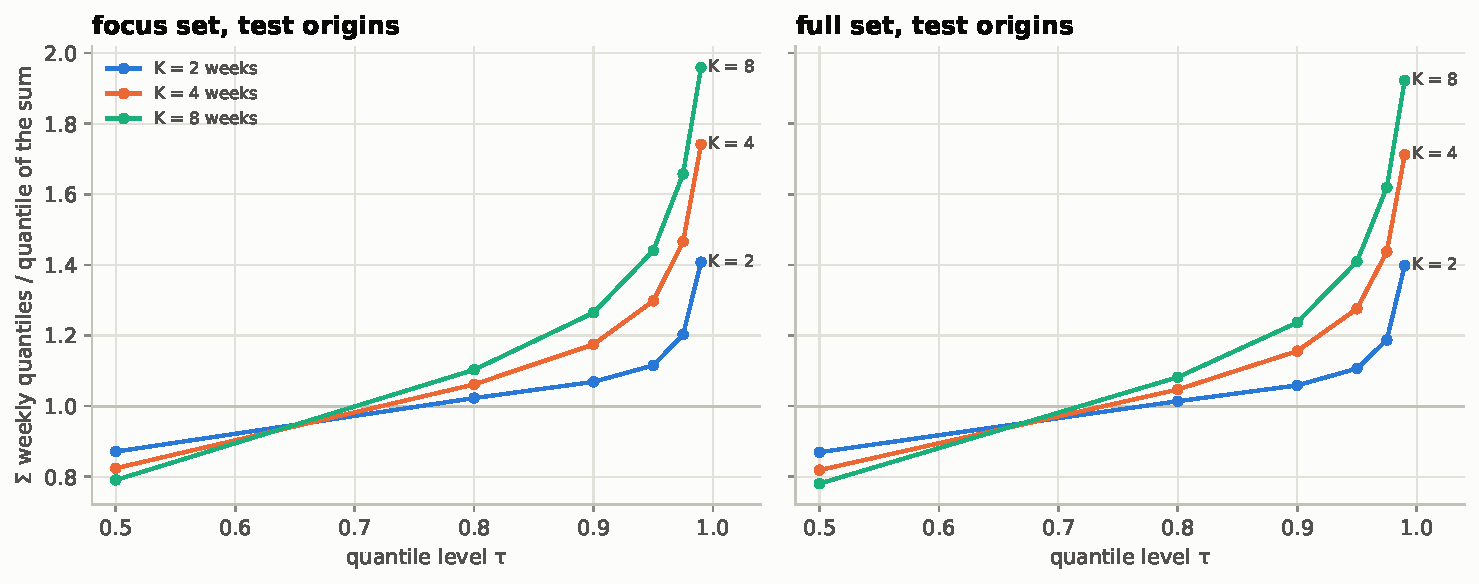
\includegraphics[width=\textwidth]{figures/horizon_sums_test.pdf}
  \caption{Sum of the weekly quantiles divided by the quantile of the sum from sample paths,
    revenue weighted, test origins (E9). Above 1: the shortcut overstates the quantile.}
  \label{fig:sums}
\end{figure}

How much the shortcut matters (Figure~\ref{fig:sums}): at $\tau = 0.95$ the summed weekly
quantiles are 12\,\%, 29\,\% and 44\,\% higher than the quantiles of the sum for $K = 2$, 4
and 8 weeks (focus set, test origins). On the test origins the summed quantiles cover 91\,\%
and 99\,\% of the 8-week sums at nominal 80 and 95\,\%; the paths cover 76\,\% and 92\,\% and
have a significantly lower CRPS ($-0.032$); independent paths (no dependence between weeks)
cover only 61\,\% and 77\,\%. The paths are slightly too narrow at long horizons, but much
closer to nominal than either shortcut. For an order-up-to policy, summed quantiles would
mean systematically more stock than intended.

\section{Final results on the test origins}
\label{sec:results}

\begin{figure}[t]
  \centering
  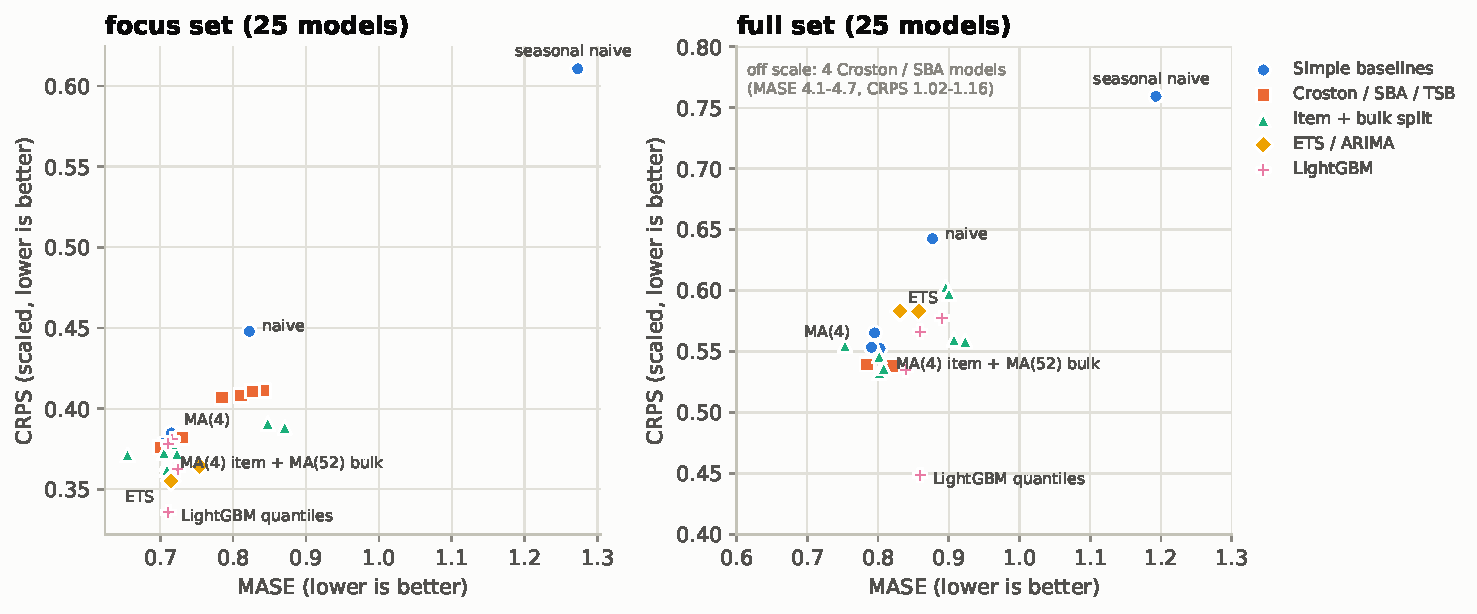
\includegraphics[width=\textwidth]{figures/models_test.pdf}
  \caption{All 25 models on the test origins: MASE (point accuracy) against CRPS (accuracy of
    the quantiles). Full set: four Croston/SBA runs lie far outside the plotted range.}
  \label{fig:models}
\end{figure}

All 25 tuning models were run once on the 26 test origins (Figure~\ref{fig:models},
Tables~\ref{tab:test-focus} and~\ref{tab:test-full} in the appendix). On the focus set the
LightGBM quantile models have the lowest CRPS of all models (0.336; next ETS with 0.355) and
a MASE of 0.711. Several simple methods reach a similar or lower plain MASE (MA(8) 0.704, TSB
0.701, MA(4) item without bulk 0.655), but they pay for it with bias (the last one ignores bulk
orders and under-forecasts by 40\,\%) and with worse quantiles. Against seasonal naive the
selected model improves MASE by $0.562$ ($-44$\,\%, CI $[-0.611, -0.512]$) and CRPS by
$0.275$; against MA(4) by $0.004$ (n.s.) and $0.049$ ($[-0.059, -0.041]$). Revenue-weighted,
the MASE gain over MA(4) is significant ($-0.033$, $[-0.053, -0.013]$).

\begin{figure}[t]
  \centering
  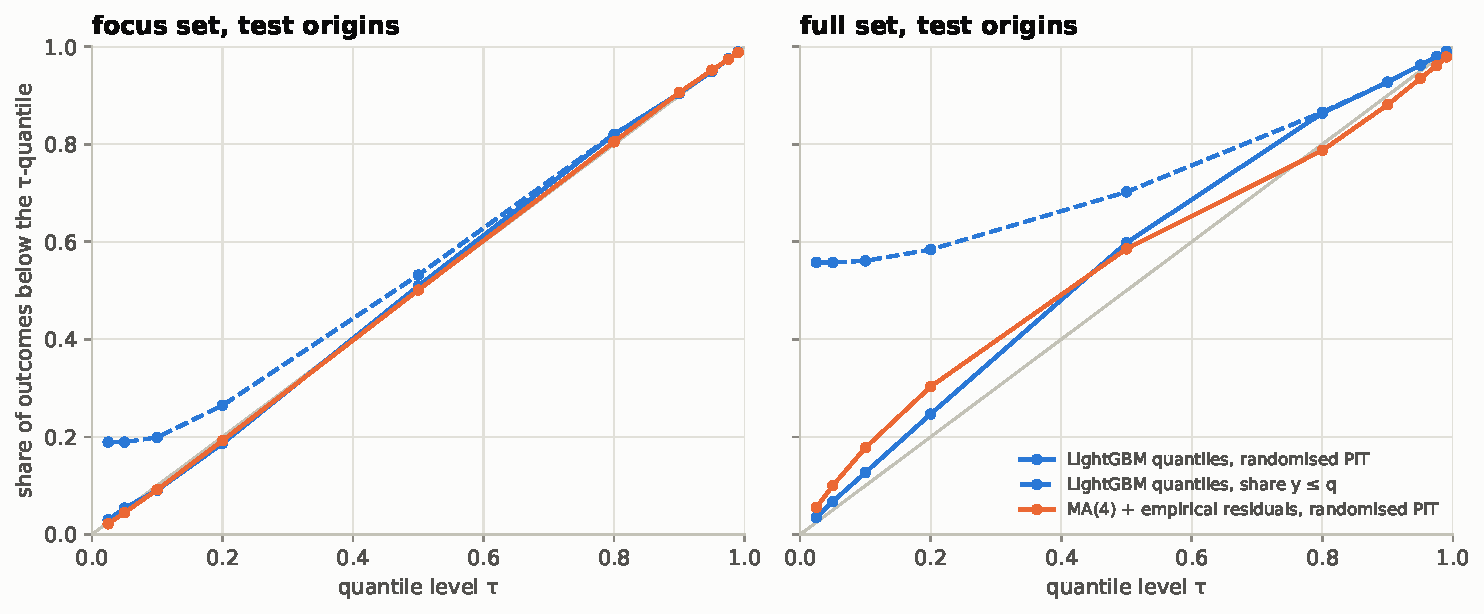
\includegraphics[width=\textwidth]{figures/calibration_test.pdf}
  \caption{Share of test outcomes below each forecast quantile. Solid: randomised PIT (ties
    counted fractionally); dashed: plain share $y \le q$, inflated by zero weeks.}
  \label{fig:calibration}
\end{figure}

\paragraph{Calibration.} Figure~\ref{fig:calibration} shows the quantiles on the test origins.
On the focus set the randomised hit rates lie on the diagonal at every level, and the central
intervals cover 81.4\,\% and 94.5\,\% (nominal 80 and 95\,\%). On the full set the lower and
middle quantiles are too high (60\,\% of the outcomes fall below the median) while the upper
levels are accurate; coverage 80.1\,\% and 94.5\,\%. The plain share $y \le q$ (dashed)
shows why the randomised PIT is needed: counted naively, the 80\,\% interval of the focus set
would ``cover'' 85\,\% of the outcomes because of zero weeks.

\paragraph{A selection that did not transfer.} On the full set the composite of the selected
models is \emph{worse} than the LightGBM quantile model alone (CRPS 0.479 vs.\ 0.449). The
cause is the unclassified products: on the tuning origins (469 of them, January--May) naive had
the lowest CRPS (0.187 vs.\ 0.234), on the test origins (572, many of them new autumn
products) LightGBM is far better (1.03 vs.\ 1.45). The selection was fixed before the test runs
and is reported as it was; the lesson is that new products behave differently in the autumn
launch season than in spring, and a selection from five spring months cannot see this.

\begin{figure}[t]
  \centering
  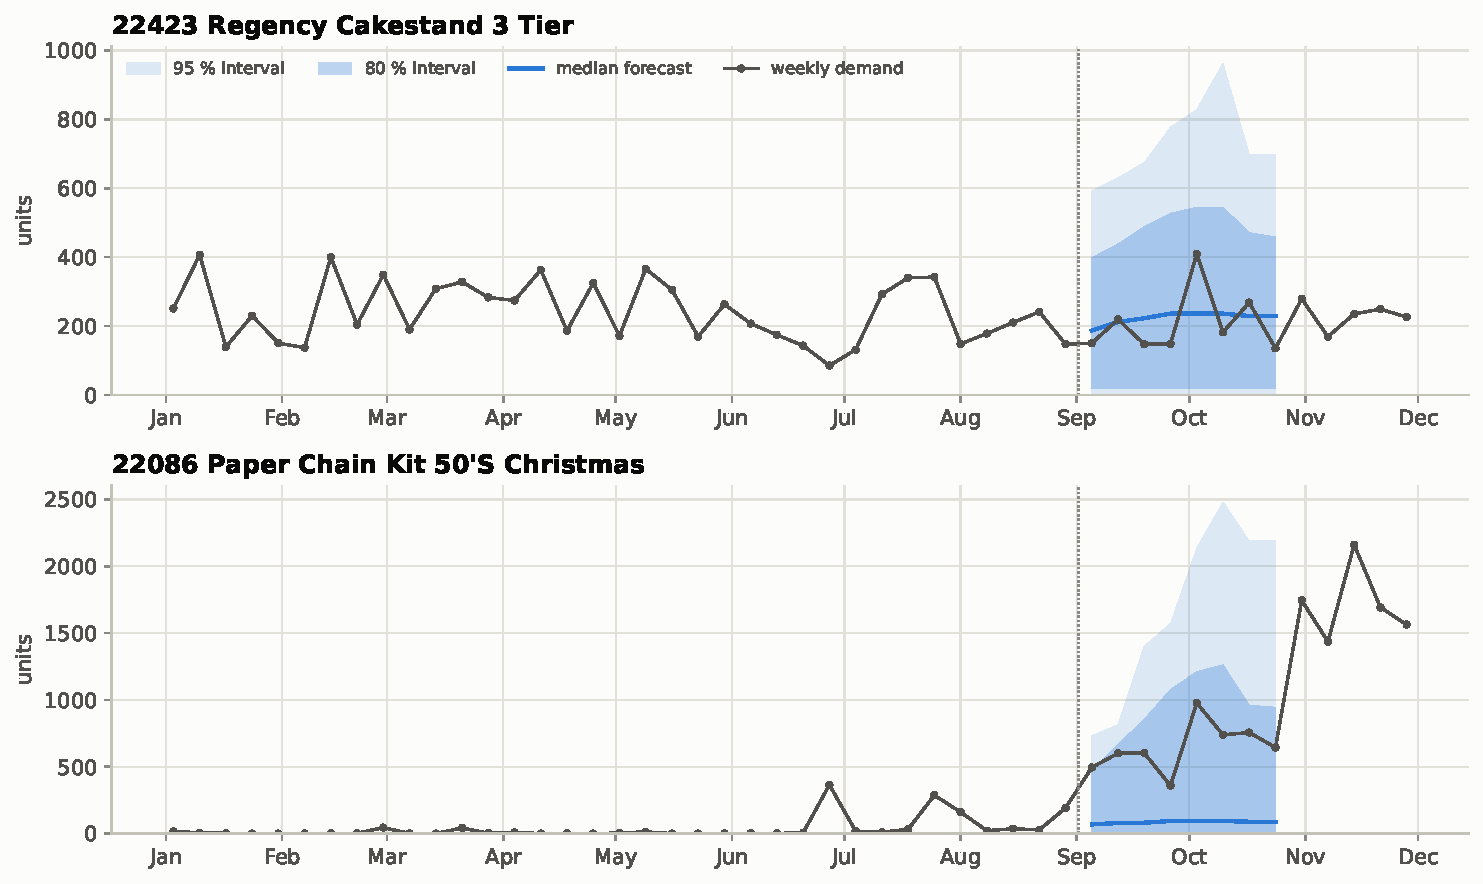
\includegraphics[width=\textwidth]{figures/fan_chart.pdf}
  \caption{Forecasts from the origin of 5 September 2011 for the largest smooth and the largest
    lumpy product of the focus set: median, 80\,\% and 95\,\% intervals, and the realised
    weekly demand.}
  \label{fig:fan}
\end{figure}

Figure~\ref{fig:fan} shows what the numbers mean for single products. For a smooth product
the median follows the level and the intervals widen into the Christmas season. For a lumpy
Christmas product the median stays low while the upper quantiles reach the demand that comes:
the model cannot know when the wholesale orders arrive, but it knows that they may, and the
order-up-to level is taken from the upper quantiles.

\section{From forecast to order quantity}
\label{sec:newsvendor}

\paragraph{One period: the newsvendor.} Before a period with random demand $D$ (distribution
function $F$) the shop stocks $S$ units. Every unit short costs $c_u$ (the lost margin), every
unit left over costs $c_o$ (holding it until it can be sold). The expected cost is
\begin{equation}
  C(S) = c_o\,\E\bigl[(S - D)^+\bigr] + c_u\,\E\bigl[(D - S)^+\bigr].
  \label{eq:newsvendor}
\end{equation}
Raising $S$ by one unit costs $c_o$ if demand ends below $S$ (probability $F(S)$) and saves
$c_u$ if it ends above (probability $1 - F(S)$). For continuous $F$ with density $f$,
\begin{equation}
  C'(S) = c_o F(S) - c_u\bigl(1 - F(S)\bigr), \qquad C''(S) = (c_u + c_o) f(S) \ge 0,
\end{equation}
so $C$ is convex and minimal where $C'(S) = 0$:
\begin{equation}
  S^* = F^{-1}(\tau^*), \qquad \tau^* = \frac{c_u}{c_u + c_o}.
  \label{eq:critical}
\end{equation}
The cost-optimal stock is a \emph{quantile} of demand, at the \emph{critical ratio} $\tau^*$.
For discrete demand the same argument with differences instead of derivatives gives the
smallest $S$ with $F(S) \ge \tau^*$, again the $\tau^*$-quantile.

\paragraph{The same loss as the forecast.} The pinball loss of Section~\ref{sec:metrics}
(unscaled) is $\rho_\tau(D, S) = \tau (D - S)^+ + (1 - \tau)(S - D)^+$. Since
$(c_u + c_o)\tau^* = c_u$ and $(c_u + c_o)(1 - \tau^*) = c_o$,
\begin{equation}
  (c_u + c_o)\,\rho_{\tau^*}(D, S) = c_u (D - S)^+ + c_o (S - D)^+ ,
  \qquad
  C(S) = (c_u + c_o)\,\E\bigl[\rho_{\tau^*}(D, S)\bigr].
\end{equation}
The business cost of a stock level \emph{is}, up to a constant, the expected pinball loss at the
critical ratio. A model trained on the pinball loss at level $\tau$ (Section~\ref{sec:models},
E5) is therefore trained on exactly the loss that the order decision minimises, and the CRPS,
the pinball loss averaged over all levels, measures the forecast for every possible cost
ratio at once. This is why the comparison of models in this report rests on the CRPS rather
than on MASE alone.

\paragraph{Many periods: periodic review, order-up-to.} The shop reviews its stock every $R$
weeks and orders arrive $L$ weeks after they are placed. At a review at the start of week $t$
the order is
\begin{equation}
  q_t = \max\bigl(0,\; S_t - \text{IP}_t\bigr), \qquad
  \text{IP}_t = \text{stock on hand} + \text{stock on order}.
\end{equation}
Nothing ordered later arrives before week $t + L + R$, so the inventory position after
ordering has to cover the demand of the $K = L + R$ weeks $t, \dots, t + K - 1$. Applying the
newsvendor argument to that sum gives
\begin{equation}
  S_t = F_t^{-1}(\tau),
\end{equation}
with $F_t$ the distribution of $D_t + \dots + D_{t+K-1}$ given the weeks before $t$: a quantile
of a \emph{sum}, which is what the sample paths of Section~\ref{sec:paths} provide.
With lost sales the multi-period problem has no closed-form optimum; the order-up-to rule
with the newsvendor level is the standard approximation (leftover stock is not lost but
carried into the next cycle, so $c_o$ is the holding cost over one review period, not the unit
cost).

\paragraph{Cost model.} The data have prices but no costs, so the costs are explicit
assumptions, kept in one file (\texttt{costs.yaml}). For a product with price $p$ (its median weekly
price before the first simulated week): unit cost $c = (1 - m)p$ with gross margin
$m = 40\,\%$; holding cost $h = r c / 52$ per unit and week with $r = 25\,\%$ per year
(capital, storage, handling); lost sales cost the margin, $c_u = m p$; $L = R = 1$ week and no
fixed order cost. Then $c_o = h R$ and the price cancels from the critical ratio:
\begin{equation}
  \tau^* = \frac{m}{m + r (1 - m) R / 52} = \frac{0.4}{0.4 + 0.25 \cdot 0.6 / 52}
  \approx 0.993 .
\end{equation}
A lost sale costs about 140 times as much as holding the unit for another week, so the
cost-optimal policy stocks for almost every eventuality. Real shops hold less, because seasonal
stock may not sell after Christmas, and because cash and space are limited. Instead of hiding
this in a single optimum, Section~\ref{sec:simulation} shows the trade-off between stock and
service as $\tau$ varies, and an optional write-down of seasonal stock (50\,\% of $c$ for the
Christmas and Easter products left at the end) is reported as a separate scenario.

\paragraph{Policies.} Three ways to set $S_t$, each from the weeks before $t$ only:
\begin{itemize}
  \item \textbf{P-naive}, the spreadsheet rule: $S_t = K \cdot \bar y_4 \cdot (1 + b)$, with
    $\bar y_4$ the mean of the last four weeks and a safety buffer $b$.
  \item \textbf{P-normal}, the textbook rule: $S_t = K \bar y_4 + z_\alpha\,\sigma \sqrt{K}$,
    with $\sigma$ the root mean square of the one-step errors of the 4-week mean over the last
    52 weeks and independent normal weeks.
  \item \textbf{P-quantile}: $S_t$ = the $\tau$-quantile of the $K$-week sums of 1\,000 sample
    paths of the LightGBM quantile forecasts made at origin $t$.
\end{itemize}

\section{Inventory simulation}
\label{sec:simulation}

\paragraph{Set-up.} Every product of the focus set is simulated week by week over the 26 test
weeks (6 June to 28 November 2011) with its observed weekly demand. At the start of each week
the orders due arrive, the order $q_t$ is placed (review period $R = 1$ week) and arrives $L$
weeks later, and the week's demand is served from stock; demand that cannot be served is lost.
The simulation starts with stock $S$ and nothing on order. Fill rate is the share of demand
served, average stock is valued at unit cost, and the total cost is holding cost plus lost
margin. Each policy is run over a grid of its parameter (P-naive buffers $b$ from 0 to 1.5,
$\alpha$ and $\tau$ from 0.5 to 0.99), fixed before the test run, so that each traces a
trade-off curve between stock and service.

\paragraph{Operating points fixed in advance.} To compare policies at single points without
choosing them on the test data, the points were fixed on the tuning weeks (28 March to
30 May 2011, after the sample-path pool has filled): two P-naive references, buffer 0 (the
plain spreadsheet rule) and buffer 1 (twice the four-week mean per review cycle, about 90\,\%
fill), and for each the smallest $\tau$ (P-quantile) and $\alpha$ (P-normal) whose tuning
fill rate reaches the reference's. For $L = 1$ these are $\tau = 0.7$ and $\tau = 0.925$; with
buffer 0, P-normal coincides with P-naive ($\alpha = 0.5$, both $K \bar y_4$).

\begin{figure}[t]
  \centering
  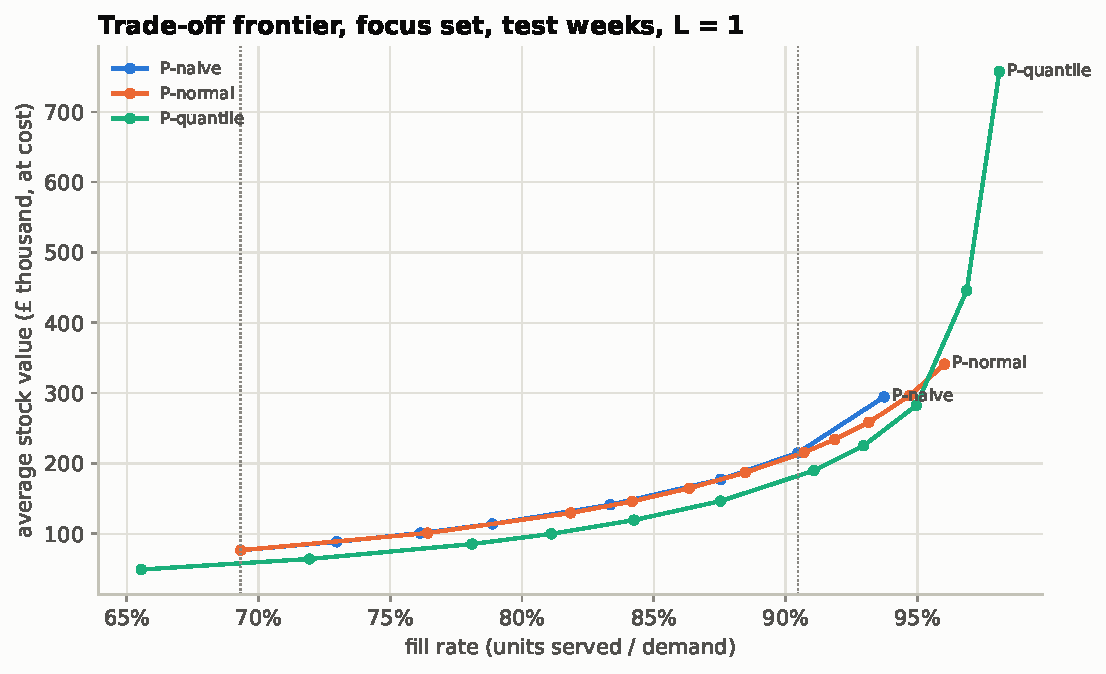
\includegraphics[width=0.8\textwidth]{figures/p5_frontier_test.pdf}
  \caption{Trade-off between average stock value and fill rate on the test weeks, lead time
    $L = 1$; each point is one grid value of a policy. Dotted: the fill rates of the two
    P-naive references.}
  \label{fig:frontier}
\end{figure}

\paragraph{Results.} Figure~\ref{fig:frontier} shows the trade-off for $L = 1$. Between about
70\,\% and 93\,\% fill rate the quantile policy needs clearly less stock than both classical
rules: at the fill rate of P-naive with buffer 0 (69.3\,\%) £58\,k instead of £77\,k, at that
of buffer 1 (90.5\,\%) £183\,k instead of £215\,k (P-normal £213\,k). With longer lead times the
gap grows: at $L = 4$ and 93\,\% fill, £389\,k against £545\,k (P-normal £469\,k).
Table~\ref{tab:policies} compares the pre-fixed operating points.

\begin{table}[ht]
  \centering
  \small
  \caption{Test weeks, operating points fixed on the tuning weeks, against their P-naive
    reference. Differences of the totals over the 748 products with paired bootstrap 95\,\%
    intervals over products; * = significant. Base costs (margin 40\,\%, holding 25\,\% per
    year).}
  \label{tab:policies}
  \begin{tabular}{llrrr}
    \toprule
    $L$ & Reference $\to$ policy & Fill rate & Avg stock value & Total cost \\
    \midrule
    1 & $b = 0$ (69.3\,\%) $\to$ $\tau = 0.7$ & $+8.8$\,pp* & $+$£8.8\,k* & $-$£89.8\,k* \\
    1 & $b = 1$ (90.5\,\%) $\to$ $\tau = 0.925$ & $+2.5$\,pp* & $+$£10.1\,k* & $-$£31.4\,k* \\
    2 & $b = 1$ (92.0\,\%) $\to$ $\tau = 0.925$ & $+1.5$\,pp* & $-$£21.6\,k* & $-$£23.1\,k* \\
    4 & $b = 1$ (93.0\,\%) $\to$ $\tau = 0.95$ & $+2.8$\,pp* & $+$£0.9\,k & $-$£35.4\,k* \\
    \midrule
    1 & $b = 1$ $\to$ P-normal $\alpha = 0.9$ & $+0.2$\,pp & $+$£0.4\,k & $-$£5.1\,k \\
    \bottomrule
  \end{tabular}
\end{table}

Because the parameter grids are coarse, the matched points overshoot the reference's fill rate
and then carry slightly more stock; the success criterion set at the start (the same or a higher fill rate with
clearly less stock \emph{or} less total cost) is met through cost at every operating point,
and through stock at equal fill rate along the whole curve. P-normal is no better than P-naive
at $L = 1$; at $L = 2$ and 4 its pre-fixed points fall short of the reference's fill rate
($-1.4$ and $-1.5$\,pp). Under every combination of margin (25, 40, 60\,\%), holding rate (15,
25, 40\,\% per year) and lead time (1, 2, 4 weeks) P-quantile is cheaper than P-naive at the
operating points: 23--29\,\% against buffer 0 and 11--31\,\% against buffer 1.

\paragraph{Where the quantile policy is expensive.} Above about 95\,\% fill rate its curve
rises steeply: $\tau = 0.99$ holds £757\,k for 98\,\% (at $L = 1$), more than twice what P-normal
holds for 96\,\%. A likely reason is that the top of each weekly quantile curve is extrapolated
beyond the highest forecast level, so lumpy products are stocked for their rare large orders. The cost-optimal $\tau^* = 0.993$ of
Section~\ref{sec:newsvendor} would therefore tie up a lot of capital; a shop owner reads the
operating point off Figure~\ref{fig:frontier} instead. The write-down of unsold seasonal stock
hits the high-stock points hardest: at $L = 4$ and a full write-down the advantage over P-naive
with buffer 1 disappears (£178\,k against £177\,k); at $L = 1$ it remains (P-quantile
£127\,k, P-naive £161\,k).

\paragraph{Tuning vs.\ test.} On the ten tuning weeks the same operating points saved 14--17\,\%
of the cost against buffer 0 and up to 14\,\% against buffer 1, with several differences not
significant. The larger gains on the test weeks probably come from the autumn build-up, where
the four-week mean lags behind rising demand while the forecasts anticipate it.

\section{Limitations}
\label{sec:limitations}

\begin{itemize}
  \item \textbf{Censored demand.} Sales are observed, demand is not: weeks in which the shop was
    out of stock show too little demand. Forecasts and service levels are therefore optimistic
    in absolute terms; comparisons between models remain fair because all face the same data.
  \item \textbf{Two years of history.} The Christmas season has been seen once before the test
    period. The models handle it through cross-product features (week of year, weeks to
    Christmas) rather than per-product seasonality, and the selection on spring origins did
    not anticipate the autumn behaviour of new products (Section~\ref{sec:results}).
  \item \textbf{Discrete, intermittent demand.} Quantile coverage needs the randomised PIT to be
    meaningful; on the full set, with most series sparse, the lower quantiles remain too low.
  \item \textbf{Price is a predictive feature}, not a causal elasticity; the models say nothing
    about what a price change would do.
\end{itemize}

\begin{itemize}
  \item \textbf{Assumed costs.} Margin, holding rate, lead time and write-down are assumptions,
    not data; the sensitivity analysis varies them, but a real shop's numbers can change the
    pound amounts considerably. The ranking of the policies did not change in any
    variant tried, except that a full write-down of seasonal stock removes the advantage at
    $L = 4$ against P-naive with buffer 1.
  \item \textbf{A simplified shop.} No minimum order quantities, pack sizes, capacity limits,
    supplier delays or fixed order costs; one price per product, fixed before the simulated
    weeks; all products start with stock $S$.
  \item \textbf{Demand is the observed sales}, so lost sales during the shop's real stock-outs
    are missing, and absolute fill rates are optimistic. All policies face the same demand, so
    the comparison between them remains fair.
  \item \textbf{26 test weeks before Christmas.} The simulation ends before the peak weeks
    and the seasonal sell-off, which the write-down scenario only approximates.
\end{itemize}

\clearpage
\appendix

\section{Abbreviations}
\label{app:glossary}

\begin{center}
\footnotesize
\begin{tabular}{@{}>{\raggedright\arraybackslash}p{0.17\textwidth} p{0.79\textwidth}@{}}
  \toprule
  ABC & Revenue classes: A = products making the top 80\,\% of revenue, B = the next 15\,\%,
        C = the rest (Section~\ref{sec:segments}). \\
  ADI & Average inter-demand interval: mean number of weeks between weeks with a sale. \\
  ARIMA & Autoregressive integrated moving average model, fitted per series. \\
  CC BY & Creative Commons Attribution licence (of the data). \\
  CI & Confidence interval; here always the 95\,\% paired bootstrap interval over series. \\
  CRPS & Continuous ranked probability score; here twice the mean scaled pinball loss over the
         quantile levels (Section~\ref{sec:metrics}). Lower is better. \\
  CV$^2$ & Squared coefficient of variation (variance / mean$^2$) of the non-zero weekly demand. \\
  cov 80, cov 95 & Coverage: share of actual weeks inside the 80\,\% or 95\,\% interval. \\
  E1--E9 & The experiments of the forecasting phase (Section~\ref{sec:models}). \\
  ETS & Exponential smoothing (error, trend, seasonality) state-space model. \\
  GBM & Gradient boosting machine (as in LightGBM, a gradient-boosted tree library). \\
  IP & Inventory position: stock on hand plus stock on order. \\
  i.i.d. & Independent and identically distributed. \\
  ISO week & Calendar week starting on Monday (ISO 8601). \\
  MA($k$), ma$k$ & Moving average over the last $k$ weeks, as a forecast. \\
  MAD & Median absolute deviation (used for the outlier rule). \\
  MASE & Mean absolute scaled error: mean absolute error divided by the in-sample error of the
         naive forecast. Below 1 = better than naive was in the past. \\
  n.s. & Not significant (the CI contains 0). \\
  P-naive, P-normal, P-quantile & The three order-up-to policies of Section~\ref{sec:newsvendor}: last-weeks mean
         times a buffer, normal safety stock, quantile of the forecast sample paths. \\
  PDF & Portable document format (of this report). \\
  PIT & Probability integral transform; rcov = coverage with a randomised PIT for discrete demand. \\
  rcov 80, rcov 95 & Randomised-PIT coverage of the 80\,\% / 95\,\% interval (Section~\ref{sec:metrics}). \\
  SB & Syntetos--Boylan demand classes (smooth, erratic, intermittent, lumpy) from ADI and CV$^2$. \\
  SBA & Syntetos--Boylan approximation: Croston's method with the bias correction
        $1 - \alpha/2$. \\
  TSB & Teunter--Syntetos--Babai method: smooths the probability of a sale instead of the interval. \\
  UCI & University of California, Irvine (Machine Learning Repository, source of the data). \\
  UK & United Kingdom. \\
  w & Revenue-weighted version of a metric (in the tables). \\
  \bottomrule
\end{tabular}
\end{center}

\section{Segments}
\label{app:segments}

\begin{figure}[ht]
  \centering
  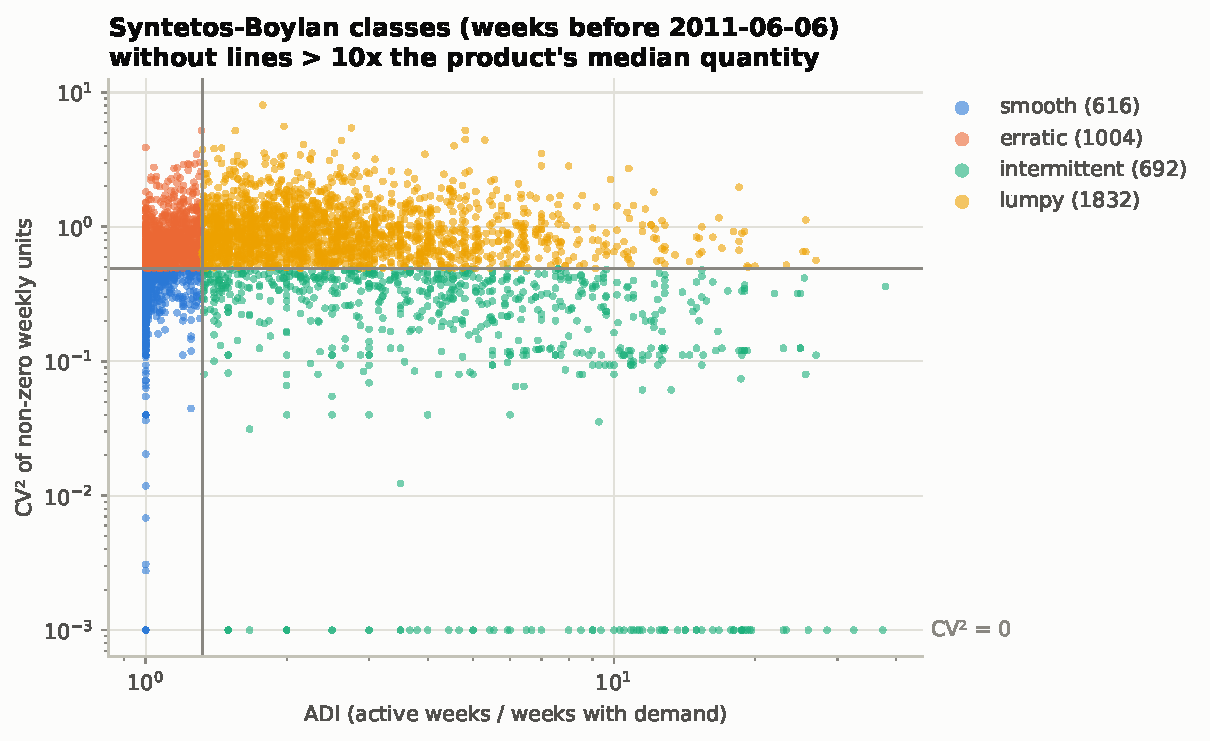
\includegraphics[width=0.7\textwidth]{figures/syntetos_boylan.pdf}
  \caption{Syntetos--Boylan classes of the products with a segment, weeks before
    6 June 2011, without lines above ten times the product's median line quantity.}
  \label{fig:sb}
\end{figure}

\begin{table}[ht]
  \centering
  \small
  \caption{Syntetos--Boylan classes (without large lines): products and revenue share; focus
    set in the last two columns.}
  \label{tab:sb}
  \begin{tabular}{lrrrr}
    \toprule
    Class & Products & Revenue & Focus products & Focus revenue \\
    \midrule
    smooth & 616 & 45.5\,\% & 293 & 39.0\,\% \\
    erratic & 1\,004 & 35.1\,\% & 373 & 24.6\,\% \\
    intermittent & 692 & 3.1\,\% & 16 & 1.2\,\% \\
    lumpy & 1\,832 & 16.3\,\% & 66 & 4.0\,\% \\
    \bottomrule
  \end{tabular}
\end{table}

\section{Full tables}
\label{app:tables}

Bias: positive = under-forecast. cov: plain share inside the interval; rcov: randomised PIT.
``w'': revenue weighted. Models with ``bulk ma52'' forecast item demand and add an MA(52) bulk
rate; ``q'' marks the LightGBM quantile models (E5).

\begin{table}[ht]
  \centering
  \footnotesize
  \setlength{\tabcolsep}{3pt}
  \caption{Tuning origins (22, January--May 2011), selected models.}
  \label{tab:tuning}
  \begin{tabular}{l rrrrr rrrrr}
    \toprule
    & \multicolumn{5}{c}{focus set} & \multicolumn{5}{c}{full set} \\
    \cmidrule(lr){2-6}\cmidrule(lr){7-11}
    Model & MASE & MASE w & bias & CRPS & rcov 80 & MASE & MASE w & bias & CRPS & rcov 80 \\
    \midrule
    naive & 0.814 & 0.836 & 0.6 & 0.442 & 83.4 & 0.711 & 0.774 & $-1.2$ & 0.493 & 76.5 \\
    seasonal naive & 1.064 & 1.027 & $-35.0$ & 0.536 & 77.2 & 1.034 & 1.005 & $-49.5$ & 0.648 & 71.3 \\
    MA(4) & 0.720 & 0.735 & 0.3 & 0.390 & 84.4 & 0.666 & 0.688 & $-3.1$ & 0.435 & 75.9 \\
    MA(8) & 0.754 & 0.784 & $-7.2$ & 0.397 & 83.8 & 0.684 & 0.734 & $-11.9$ & 0.423 & 75.7 \\
    Croston $\alpha$ 0.2 & 0.830 & 0.828 & $-14.7$ & 0.401 & 82.7 & 3.648 & 0.898 & $-67.6$ & 0.715 & 71.7 \\
    SBA $\alpha$ 0.2 & 0.784 & 0.782 & $-3.3$ & 0.397 & 82.4 & 3.321 & 0.842 & $-50.9$ & 0.683 & 71.6 \\
    TSB $\alpha$ 0.2 & 0.761 & 0.786 & $-11.5$ & 0.386 & 83.7 & 0.698 & 0.747 & $-18.3$ & 0.408 & 76.0 \\
    MA(4) item, no bulk & 0.629 & 0.637 & 34.9 & 0.366 & 83.6 & 0.601 & 0.596 & 29.3 & 0.419 & 75.1 \\
    MA(4) + bulk ma52 & 0.732 & 0.737 & $-12.8$ & 0.364 & 85.6 & 0.699 & 0.720 & $-24.3$ & 0.414 & 77.1 \\
    TSB 0.2 + bulk ma52 & 0.786 & 0.798 & $-20.4$ & 0.372 & 84.5 & 0.736 & 0.784 & $-33.8$ & 0.400 & 77.2 \\
    top-down MA(4) + bulk & 0.821 & 0.819 & $-21.7$ & 0.375 & 85.1 & 0.758 & 0.802 & $-23.1$ & 0.399 & 80.0 \\
    ETS + bulk ma52 & 0.764 & 0.762 & $-18.7$ & 0.378 & 82.9 & 0.767 & 0.743 & $-30.9$ & 0.506 & 76.1 \\
    ARIMA + bulk ma52 & 0.808 & 0.810 & $-26.5$ & 0.380 & 83.0 & 0.779 & 0.786 & $-37.9$ & 0.495 & 76.3 \\
    LightGBM item + bulk & 0.730 & 0.736 & $-12.6$ & 0.353 & 81.5 & 0.716 & 0.720 & $-24.5$ & 0.400 & 72.5 \\
    LightGBM total, p 1.5 & 0.692 & 0.685 & 2.1 & 0.357 & 81.4 & 0.709 & 0.661 & $-5.7$ & 0.411 & 72.7 \\
    LightGBM total, p 1.8 & 0.686 & 0.678 & 1.5 & 0.354 & 81.7 & 0.683 & 0.651 & $-5.0$ & 0.408 & 72.2 \\
    LightGBM total q & 0.686 & 0.678 & 1.5 & \textbf{0.339} & 80.0 & 0.683 & 0.651 & $-5.0$ & \textbf{0.357} & 77.5 \\
    \bottomrule
  \end{tabular}
\end{table}

\begin{table}[ht]
  \centering
  \footnotesize
  \setlength{\tabcolsep}{4pt}
  \caption{Test origins (26, June--November 2011), focus set, all models.}
  \label{tab:test-focus}
  \begin{tabular}{l rrrrr rrrr}
    \toprule
    Model & MASE & MASE w & bias & CRPS & CRPS w & cov 80 & cov 95 & rcov 80 & rcov 95 \\
    \midrule
    naive & 0.822 & 0.993 & 8.5 & 0.448 & 0.520 & 84.4 & 95.8 & 80.5 & 94.6 \\
    seasonal naive & 1.273 & 1.304 & $-41.2$ & 0.611 & 0.609 & 80.1 & 95.0 & 75.0 & 92.4 \\
    MA(4) & 0.715 & 0.862 & 9.0 & 0.385 & 0.444 & 85.5 & 96.5 & 81.4 & 95.2 \\
    MA(8) & 0.704 & 0.850 & 10.2 & 0.378 & 0.438 & 86.9 & 96.8 & 82.8 & 95.6 \\
    MA(13) & 0.719 & 0.867 & 10.9 & 0.385 & 0.448 & 87.4 & 96.9 & 83.3 & 95.7 \\
    Croston $\alpha$ 0.1 & 0.842 & 0.919 & 4.2 & 0.411 & 0.462 & 85.6 & 96.3 & 80.6 & 94.2 \\
    Croston $\alpha$ 0.2 & 0.811 & 0.897 & 5.9 & 0.408 & 0.455 & 85.3 & 96.2 & 80.4 & 94.3 \\
    SBA $\alpha$ 0.1 & 0.826 & 0.907 & 9.0 & 0.411 & 0.462 & 85.6 & 96.3 & 80.5 & 94.1 \\
    SBA $\alpha$ 0.2 & 0.785 & 0.877 & 15.3 & 0.407 & 0.454 & 85.4 & 96.2 & 80.2 & 94.2 \\
    TSB 0.1 & 0.730 & 0.864 & 8.3 & 0.382 & 0.444 & 87.4 & 96.9 & 83.4 & 95.7 \\
    TSB 0.2 & 0.701 & 0.841 & 9.8 & 0.376 & 0.435 & 86.7 & 96.7 & 82.7 & 95.5 \\
    MA(4) item, no bulk & 0.655 & 0.807 & 40.2 & 0.371 & 0.427 & 86.1 & 96.8 & 81.4 & 95.3 \\
    MA(4) + bulk ma52 & 0.709 & 0.824 & 2.9 & 0.366 & 0.415 & 87.1 & 96.9 & 83.0 & 95.7 \\
    MA(4) + bulk TSB 0.1 & 0.705 & 0.816 & 5.8 & 0.373 & 0.422 & 87.3 & 96.9 & 83.5 & 95.8 \\
    TSB 0.2 + bulk ma52 & 0.723 & 0.841 & 3.4 & 0.372 & 0.425 & 87.7 & 97.1 & 83.6 & 95.8 \\
    TSB 0.2 + bulk TSB 0.1 & 0.717 & 0.831 & 6.3 & 0.379 & 0.432 & 87.5 & 96.9 & 83.7 & 95.8 \\
    MA(4) + bulk, category pool & 0.709 & 0.824 & 2.9 & 0.362 & 0.410 & 87.2 & 96.9 & 83.1 & 95.7 \\
    top-down MA(4) + bulk & 0.871 & 0.956 & $-14.5$ & 0.388 & 0.434 & 86.2 & 96.9 & 81.0 & 94.7 \\
    top-down MA(13) + bulk & 0.848 & 0.938 & $-8.5$ & 0.391 & 0.441 & 87.8 & 97.3 & 82.6 & 95.3 \\
    ETS + bulk ma52 & 0.715 & 0.824 & 2.3 & 0.355 & 0.394 & 87.9 & 96.6 & 82.5 & 94.9 \\
    ARIMA + bulk ma52 & 0.754 & 0.858 & $-0.2$ & 0.364 & 0.405 & 88.3 & 96.7 & 82.5 & 94.9 \\
    LightGBM item + bulk & 0.724 & 0.835 & $-3.0$ & 0.362 & 0.417 & 79.0 & 93.3 & 74.7 & 91.6 \\
    LightGBM total, p 1.5 & 0.717 & 0.833 & 1.1 & 0.381 & 0.439 & 76.4 & 92.2 & 72.4 & 90.5 \\
    LightGBM total, p 1.8 & 0.711 & 0.829 & 0.7 & 0.378 & 0.436 & 76.5 & 92.2 & 72.5 & 90.4 \\
    LightGBM total q (selected) & 0.711 & 0.829 & 0.7 & \textbf{0.336} & \textbf{0.391} & 85.1 &
      97.5 & 81.4 & 94.5 \\
    \bottomrule
  \end{tabular}
\end{table}

\begin{table}[ht]
  \centering
  \footnotesize
  \setlength{\tabcolsep}{4pt}
  \caption{Test origins, full set, selected models. ``Composite'': the model per segment fixed
    on the tuning origins (LightGBM q, naive for unclassified products).}
  \label{tab:test-full}
  \begin{tabular}{l rrrrr rrrr}
    \toprule
    Model & MASE & MASE w & bias & CRPS & CRPS w & cov 80 & cov 95 & rcov 80 & rcov 95 \\
    \midrule
    naive & 0.877 & 1.040 & 9.0 & 0.642 & 0.580 & 79.7 & 93.5 & 71.0 & 90.4 \\
    seasonal naive & 1.193 & 1.357 & $-30.9$ & 0.759 & 0.674 & 78.9 & 94.0 & 68.5 & 89.7 \\
    MA(4) & 0.795 & 0.906 & 10.8 & 0.565 & 0.496 & 80.6 & 94.2 & 70.3 & 90.6 \\
    MA(8) & 0.791 & 0.896 & 13.0 & 0.553 & 0.491 & 81.6 & 94.9 & 70.8 & 91.2 \\
    Croston $\alpha$ 0.2 & 4.486 & 0.999 & $-17.6$ & 1.068 & 0.521 & 79.8 & 93.9 & 66.9 & 88.4 \\
    SBA $\alpha$ 0.2 & 4.102 & 0.974 & $-5.8$ & 1.019 & 0.521 & 79.7 & 93.8 & 66.7 & 88.3 \\
    TSB 0.2 & 0.784 & 0.888 & 12.9 & 0.540 & 0.487 & 82.4 & 95.1 & 71.2 & 91.3 \\
    MA(4) item, no bulk & 0.753 & 0.853 & 35.9 & 0.555 & 0.483 & 80.7 & 94.3 & 70.2 & 90.5 \\
    MA(4) + bulk ma52 & 0.802 & 0.880 & 6.4 & 0.546 & 0.471 & 82.0 & 94.6 & 71.8 & 91.0 \\
    TSB 0.2 + bulk ma52 & 0.808 & 0.899 & 7.7 & 0.536 & 0.481 & 83.6 & 95.4 & 72.7 & 91.8 \\
    ETS + bulk ma52 & 0.831 & 0.884 & 4.3 & 0.583 & 0.444 & 90.2 & 95.6 & 75.9 & 91.8 \\
    ARIMA + bulk ma52 & 0.857 & 0.915 & 3.6 & 0.583 & 0.452 & 90.2 & 95.5 & 75.7 & 91.6 \\
    LightGBM item + bulk & 0.839 & 0.893 & $-4.1$ & 0.535 & 0.467 & 77.8 & 93.0 & 65.8 & 88.0 \\
    LightGBM total, p 1.8 & 0.859 & 0.891 & $-2.1$ & 0.566 & 0.488 & 76.6 & 92.6 & 64.6 & 87.5 \\
    LightGBM total q & 0.859 & 0.891 & $-2.1$ & \textbf{0.449} & \textbf{0.426} & 90.4 & 98.0 &
      80.1 & 94.5 \\
    Composite (selected) & 0.852 & 0.893 & 1.4 & 0.479 & 0.435 & 87.4 & 96.2 & 77.1 & 92.8 \\
    \bottomrule
  \end{tabular}
\end{table}

\end{document}
